\documentclass[a4paper,10pt]{article}
\usepackage[utf8]{inputenc}

\usepackage{float}
\usepackage{graphicx}
\usepackage{float}
\usepackage{amsmath}
\usepackage{gensymb}
\usepackage{hyperref}

%opening
\title{Homework 1 - Robot Dynamics and Control}
\author{Erivelton Gualter dos Santos}

\begin{document}
\date{}
\maketitle

\section{Article summary}
\begin{center}
 Supernumerary Robotic Limbs for Human Body Support \cite{parietti2016supernumerary} \\
 F. Parietti and H.H. Asada
\end{center}

The journal paper introduces a new wearable device to support a person in dangerous and repetitive tasks, such as, carrying heavy loads in a working environment. Motivation boils down to the fact that there are several activities which is still not easily to be replaced by robots due to the slow learning rate of complex tasks. Therefore, a new device, called \textit{Supernumerary Robotic Limbs}  SRL, is proposed and it is characterized as a wearable robot to maximize the human performance. Additionally, a studying of body support stability is presented by take in consideration the stiffness matrix evaluation. 

The SRL system illustrated in Fig. \ref{fig:SRL_concept} consist on: two robotics limbs; a harness to protect the hip bone; and a control unit. The device provides support to the user without constraining its motion with the help of the three links: one prismatic joint and two revolute joints, consequently, three degrees of freedom (DOFs). According to kinematic arrangements of manipulators in \cite{spong2006robot}, the SRL system is observed to be a system with two RRP robot. 

\begin{figure}[H]
 \begin{minipage}{.5\textwidth}
  \centering
  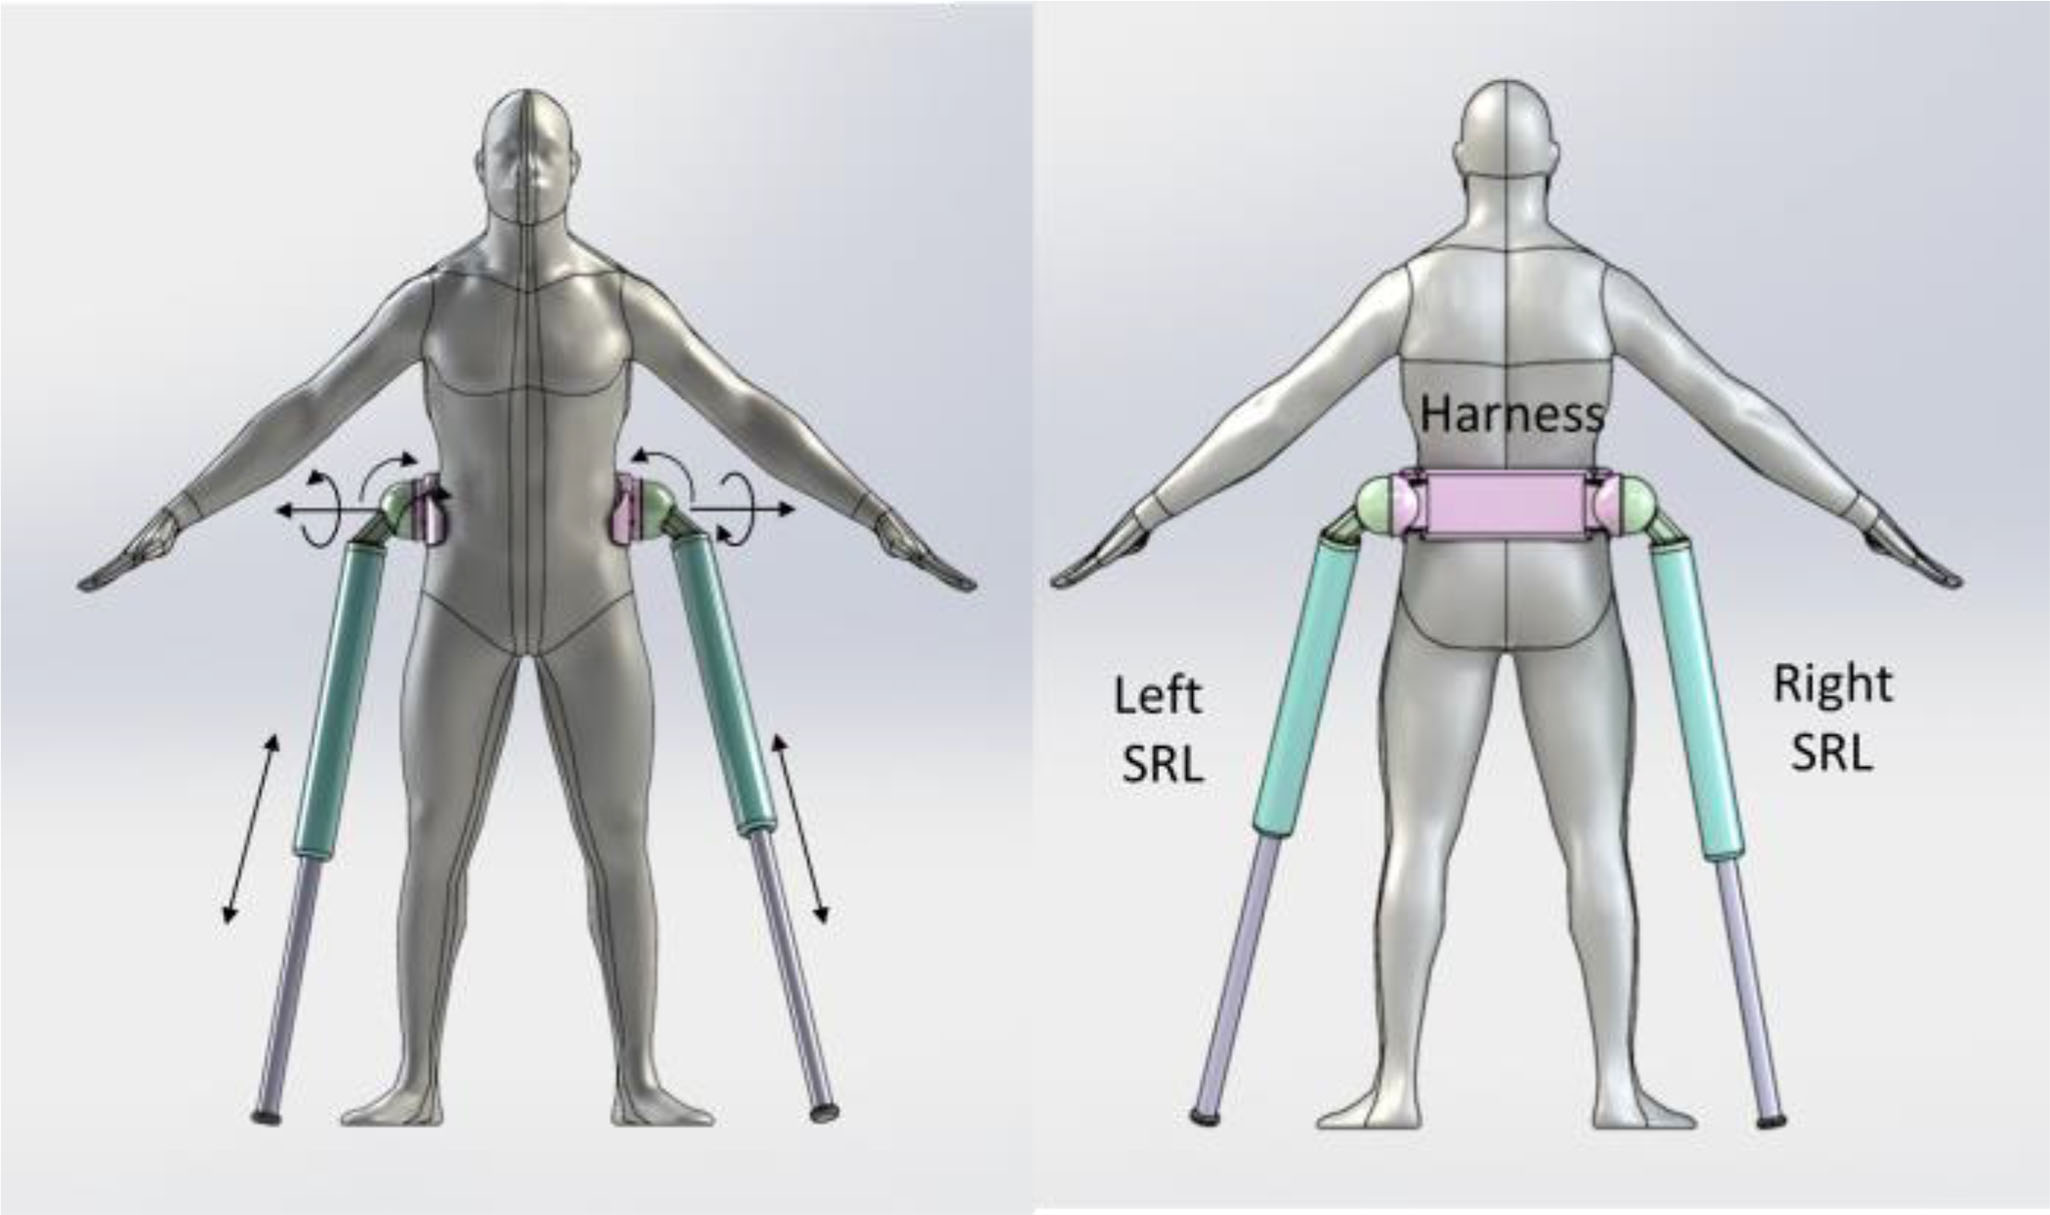
\includegraphics[height=3.5cm]{SRL_concept.png}
  \caption{Design concept of SRL.} \label{fig:SRL_concept}
 \end{minipage}
 \begin{minipage}{.5\textwidth}
  \centering
  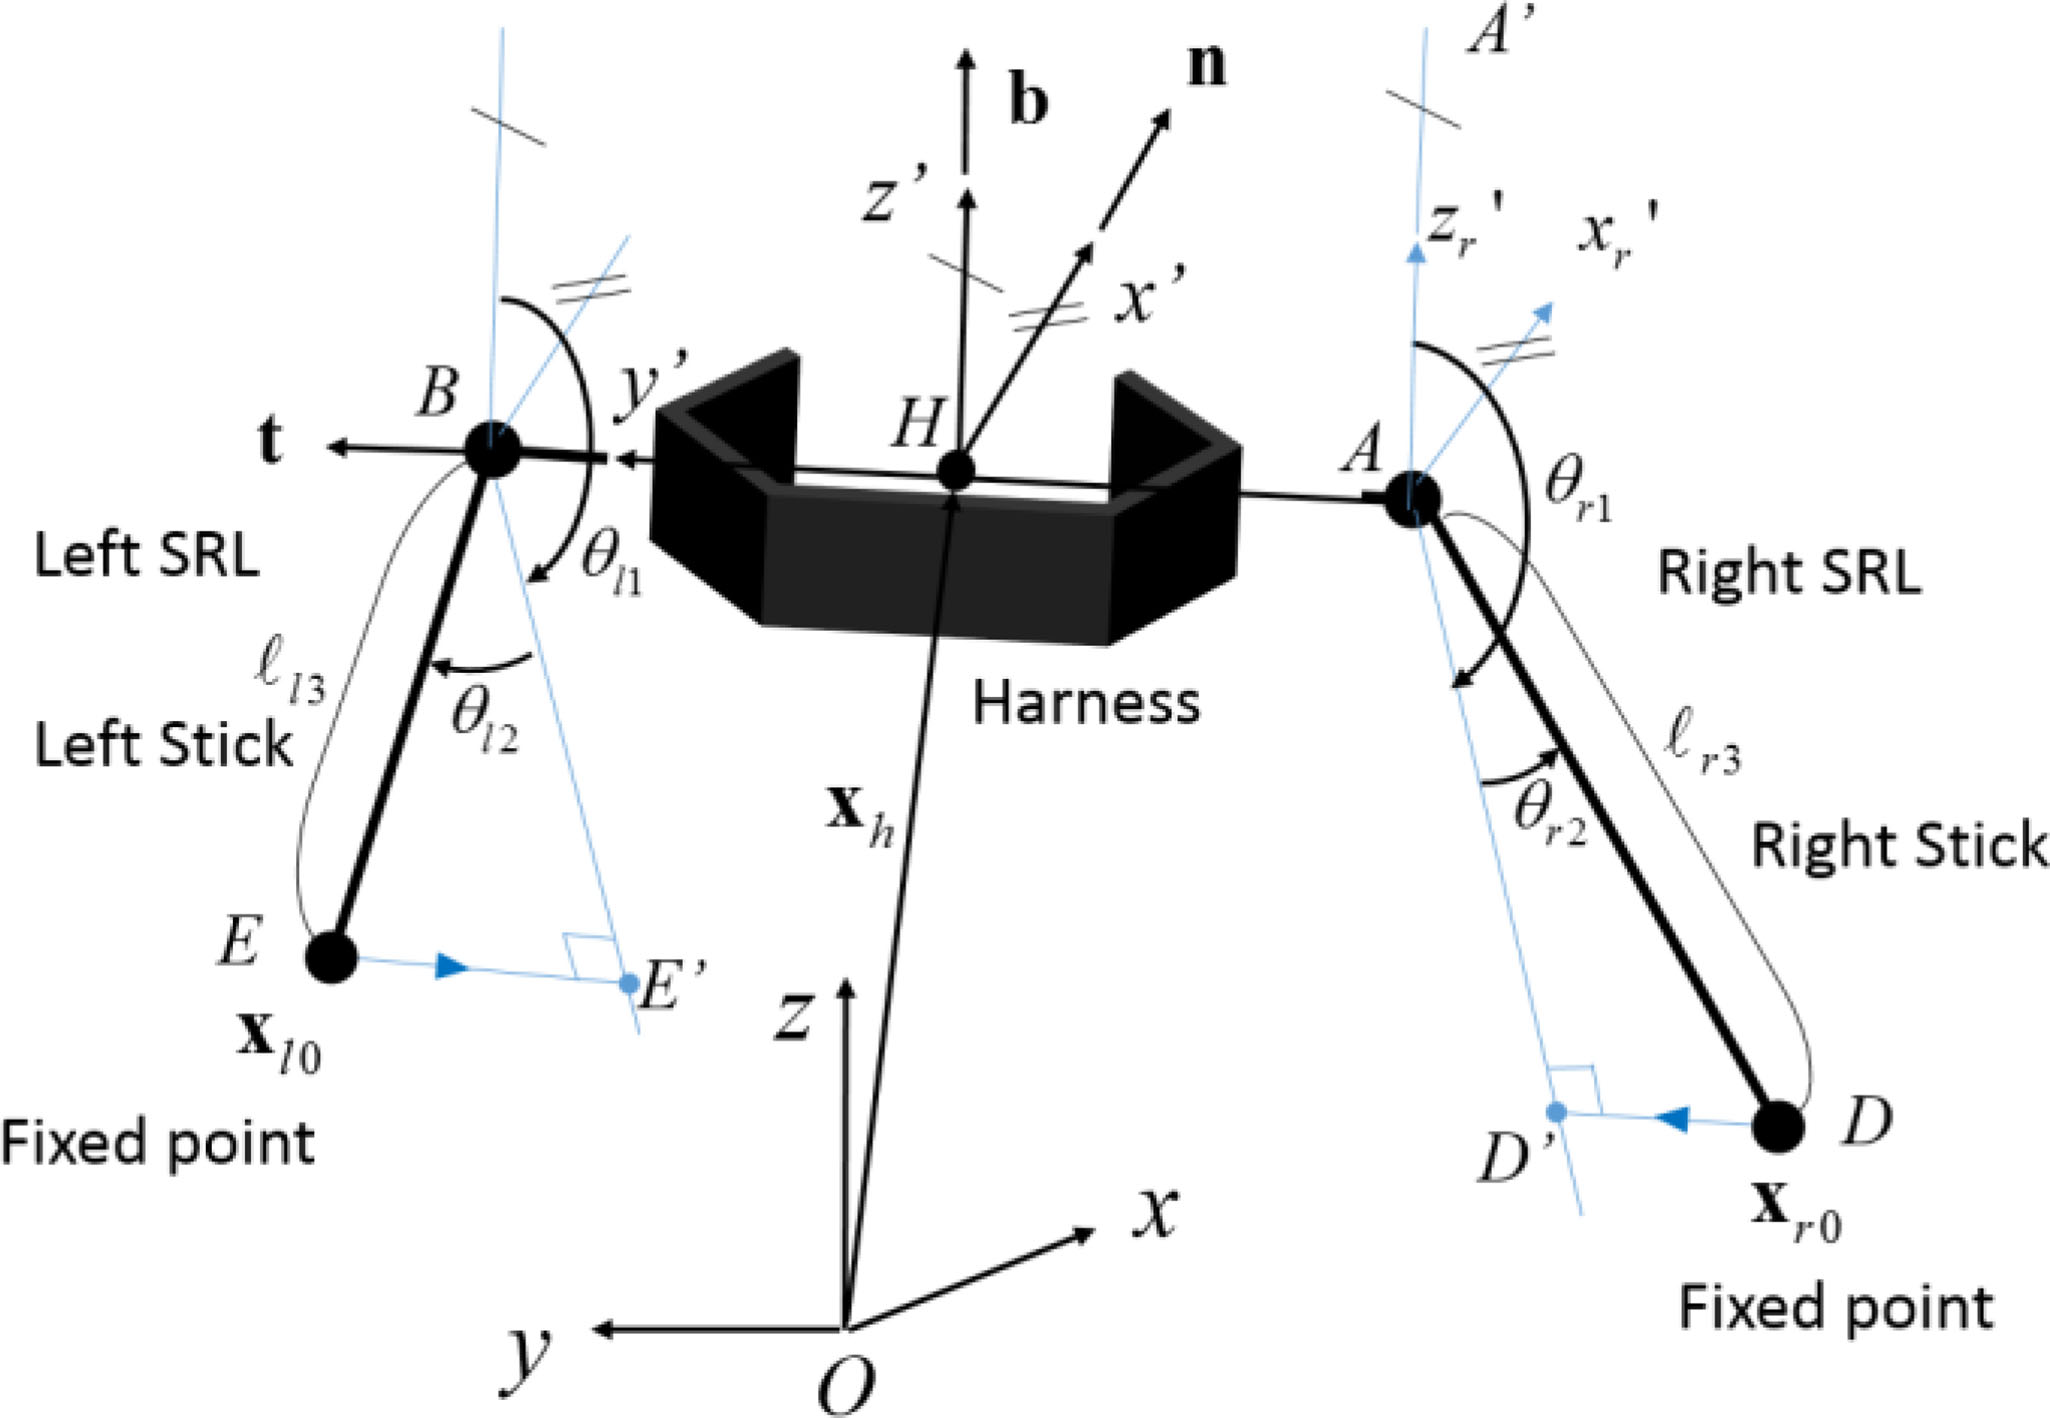
\includegraphics[height=3.5cm]{SRL_schematic.png}
  \caption{Schematic of the SRL system.} \label{fig:SRL_schematic}
 \end{minipage}
\end{figure}

In order to study the support stability, the forward kinematic is presented, in additional, the differentiation of its equation results in Jacobian Matrix. Some assumptions are made by the authors, such as, massless of the SRL links and center of the mass equivalent to the center of the human body in combination with the harness. 

The authors conclude the work by provind the SRL design works weel. A prototype was built and tested in diferent working environments. Additionally two control techniques presented and demostrated sucess to stabilize the body support: 
\begin{itemize}
 \item Null-space stabilization using Hessian;
 \item Joint servo stiffness control based on the Jacobian. 
\end{itemize}


\bibliography{ref_hw1} 
\bibliographystyle{ieeetr}

\section{Question 2}

The figure shows two planar manipulators of the RP and PR
types. For each, write Matlab code that displays the reachable workspace for
a given set of parameters. Show the shape of the reachable workspaces for
the following parameter values: $l_1 = l_2 = 1$, $\delta = 0.2$, $d = 0.2$, $h = 0.5$ and $D = 0.75$.

\hfill \break
\textbf{RP robot}: The range of motion of the prismatic link is $0 \leq q_2 \leq≤ D$. The
range of motion of the revolute joint is limited by interference between
the first link and the ground and between the end effector and the ground.

\begin{figure}[H]
  \centering
  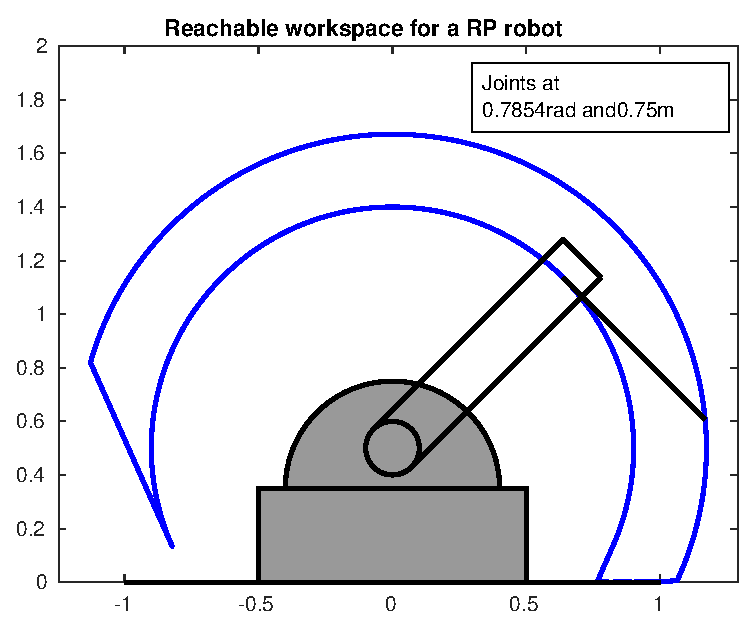
\includegraphics[width=.6\linewidth]{rprobot.eps}
  \caption{Reachable Workspace.} \label{fig:rp}
\end{figure}

\hfill \break
\textbf{PR robot}: The range of motion of the prismatic link is  $0 \leq q_1 \leq≤ D$. The range of
motion of the revolute joint is limited only by intereference between the
end effector and the ground

\begin{figure}[H]
  \centering
  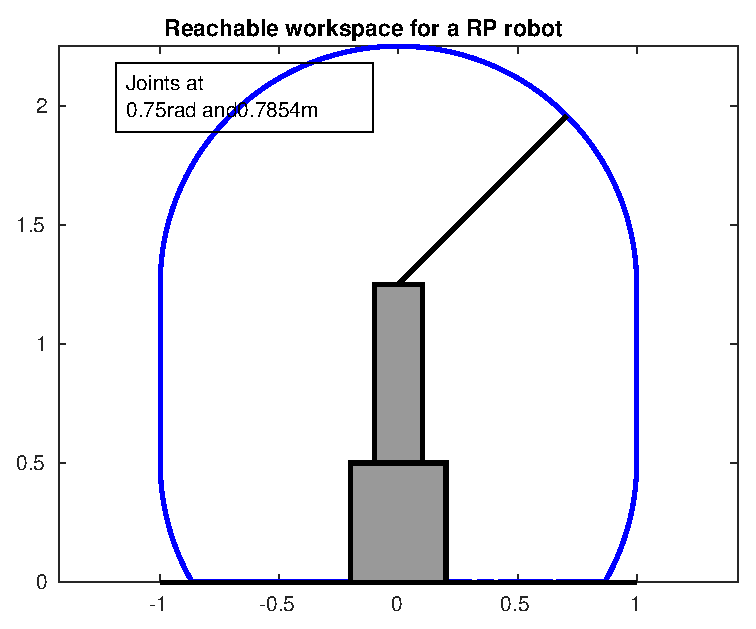
\includegraphics[width=.6\linewidth]{prrobot.eps}
  \caption{Reachable Workspace} \label{fig:pr}
\end{figure}

\section{Code Instruction}

\begin{itemize}
 \item Download the code (\textbf{MAINroboticsHW1.m}) attached in the email. 
 \item Alternatively, the code is avaliable at \url{https://github.com/EriveltonGualter/MCE747-Robot-Dynamics-and-Control} after submission deadline.
 \item Run MAINroboticsHW1.m 
\end{itemize}



% \section{Question 3}
% 
% \begin{enumerate}
%  \setcounter{enumi}{2}
%  \item \textbf{Set 2.1:} Describe the column space and the nullspace of the matrices.
% \end{enumerate}
% 
% \begin{center}
%  $A=
% \begin{bmatrix}
% 1 & -1 \\
% 0 & 0
% \end{bmatrix}
% $and $B = 
% \begin{bmatrix}
% 0 & 0 & 3 \\
% 1 & 2 & 3
% \end{bmatrix}
% $and $C = 
% \begin{bmatrix}
% 0 & 0 & 0 \\
% 0 & 0 & 0
% \end{bmatrix}$
% \end{center}
% 
% For $A = \left[\begin{array}{cc} 1 & -1\\ 0 & 0 \end{array}\right]$ we know:
% 
% \begin{equation*}
%   Col(A) = span \left\lbrace \left[\begin{array}{c} 1 \\ 0 \end{array}\right] , \left[\begin{array}{c} -1\\ 0 \end{array}\right]\right\rbrace  = \left\lbrace C_1\left[\begin{array}{c} 1 \\ 0 \end{array}\right] + C_2 \left[\begin{array}{c} -1\\ 0 \end{array}\right]\right\rbrace
% \end{equation*}
% 
% 
% Therefore, we have only a dimension which correspond to the abscissa.
% 
% The solution to $Ax = 0$ form a vector space, which correspond to the \textbf{nullspace} of $A$. Then:
% 
% \begin{eqnarray*}
% \begin{bmatrix}
% 1 & -1 \\
% 0 & 0
% \end{bmatrix} 
% \begin{bmatrix}
% x_1 \\ x_2
% \end{bmatrix}  = 0
% \end{eqnarray*}
% 
% It results in: $x_1 = x_2$
% 
% \begin{figure}[H]
%   \centering
%   \includegraphics[width=.6\linewidth]{prob2_1a.eps}
%   \caption{Column and Nullspace representation of A.} \label{fig:prob2_1a}
% \end{figure}
% 
% For $B = \left[\begin{array}{ccc} 0 & 0 & 3\\ 1 & 2 & 3 \end{array}\right]$:
% 
% \begin{equation*}
%   Col(B) = span \left\lbrace \left[\begin{array}{c} 0 \\ 1 \end{array}\right], \left[\begin{array}{c} 0 \\ 2 \end{array}\right] , \left[\begin{array}{c} 3\\ 3 \end{array}\right]\right\rbrace  = C_1\left\lbrace \left[\begin{array}{c} 1 \\ 0 \end{array}\right] + C_2 \left[\begin{array}{c} -1\\ 0 \end{array}\right]\right\rbrace
% \end{equation*}
% 
% %$Col (A) = span \left\lbrace \right\rbrace $
% \begin{enumerate}
%  \setcounter{enumi}{7}
%  \item \textbf{Set 2.1:} Which of the following descriptions are correct? The solutions x of form
% \end{enumerate}
% 
% \begin{equation*}
%  Ax = 
%  \begin{bmatrix}
%   1 & 1 & 1 \\
%   1 & 0 & 2 
%  \end{bmatrix} 
%  \begin{bmatrix}
%   x_1\\x_2\\x_3
%  \end{bmatrix} = 
%  \begin{bmatrix}
%   0\\0
%  \end{bmatrix}
% \end{equation*}
% 
% 
% \begin{enumerate}
% \setcounter{enumi}{16}
%  \item \textbf{Set 2.1:} The four types of subspaces of $\textbf{R}^3$ are planes, lines, $\textbf{R}^3$ itself, or $\textbf{Z}$ containing only $(0,0,0)$.
%  \begin{enumerate}
%   \item Describe the three types of subspaces of $\textbf{R}^2$.
%   \item Describe the five types of subspaces of $\textbf{R}^4$.
%  \end{enumerate}
% \end{enumerate}
% 
% \begin{enumerate}
% \setcounter{enumi}{1}
% \item \textbf{Set 2.3:} Find the largest possible number of independent vectors among
% \end{enumerate}
% 
% 
% \begin{equation*}
%  v_1 = 
%  \begin{bmatrix}
%   1 \\ -1\\ 0 \\0
%  \end{bmatrix} \:\:
%   v_2 = 
%  \begin{bmatrix}
%   1 \\ 0\\ -1 \\0
%  \end{bmatrix} \:\:
%   v_3 = 
%  \begin{bmatrix}
%   1 \\ 0\\ 0 \\-1
%  \end{bmatrix} \:\:
%   v_4 = 
%  \begin{bmatrix}
%   0 \\ 1\\ -1 \\0
%  \end{bmatrix} \:\:
%   v_5 = 
%  \begin{bmatrix}
%   0 \\ 1\\ 0 \\-1
%  \end{bmatrix} \:\:
%    v_6 = 
%  \begin{bmatrix}
%   0 \\ 0\\ 1 \\-1
%  \end{bmatrix} \:\:
% \end{equation*}
% 
% \begin{enumerate}
% \setcounter{enumi}{19}
% \item \textbf{Set 2.3:} Find a basis for each of these subspaces of $\textbf{R}^4$:
% \begin{enumerate}
%  \item All vectors whose components are equal.
%  \item All vectors whose components add to zero.
%  \item All vectors that are perpendicular to $(1, 1, 0, 0)$ and $(1, 0, 1, 1)$.
%  \item The column space (in $\textbf{R}^2$) and nullspace (in $\textbf{R}^5$ ) of $U = \begin{bmatrix}
% 1 & 0 & 0 & 1 & 1 \\ 
% 0 & 0 & 1 & 1 & 0                                                                                       \end{bmatrix}$
% \end{enumerate}
% \end{enumerate}
% 
% \begin{enumerate}
% \setcounter{enumi}{30}
% \item \textbf{Set 2.3:} Find a counterexample to the following statement: If $v_1$, $v_2$, $v_3$, $v_4$ is a basis for the
% vector space $\textbf{R}^4$, and if $\textbf{W}$ is a subspace, then some subset of the v’s is a basis for $\textbf{W}$.
% \end{enumerate}
% 
% \begin{enumerate}
%  \setcounter{enumi}{4}
%  \item \textbf{Set 2.6:} The matrix $A = \begin{bmatrix}
%                                           1 & 0\\3 & 1
%                                          \end{bmatrix}
% $ yields a shearing transformation, which leaves the y-axis unchanged. Sketch its effect on the x-axis, by indicating what happens to $(1, 0)$ and $(2, 0)$ and $(−1, 0)$ — and how the whole axis is transformed
% \end{enumerate}
% 
% \begin{enumerate}
%  \setcounter{enumi}{5}
%  \item \textbf{Set 2.6:} What 3 by 3 matrices represent the transformations that
%  \begin{itemize}
%   \item project every vector onto the x-y plane?
%   \item reflect every vector through the x-y plane?
%   \item rotate the x-y plane through $90\degree$ , leaving the z-axis alone?
%   \item rotate the x-y plane, then x-z, then y-z, through $90\degree$?
%   \item carry out the same three rotations, but each one through $180\degree$ ?
%  \end{itemize}
% \end{enumerate}
% 
% \begin{enumerate}
%  \setcounter{enumi}{6}
%  \item \textbf{Set 2.6:} On the space $\textbf{P}_3$ of cubic polynomials, what matrix represents $d_2/d_{t^2}$? Construct
% the 4 by 4 matrix from the standard basis $1$, $t$, $t^2$ , $t^3$ . Find its nullspace and column
% space. What do they mean in terms of polynomials?
% \end{enumerate}

\end{document}
